\documentclass[11pt]{article}
\usepackage[review]{acl}
\usepackage{times}
\usepackage{latexsym}
\usepackage[T1]{fontenc}
\usepackage[utf8]{inputenc}

\usepackage{amsmath}
\usepackage{amssymb}
\usepackage{graphicx}
\usepackage{subcaption}
\usepackage{booktabs}
\usepackage{microtype}
\usepackage{array}
\usepackage{algorithm}
\usepackage{algorithmic}

% Fix line numbers: always place on outer margins (left margin for col 1,
% right margin for col 2). ACL's default [switch] places them in the gap.
\makeatletter
\AtBeginDocument{%
  \def\makeLineNumber{%
    \if@firstcolumn
      \makeLineNumberLeft
    \else
      \makeLineNumberRight
    \fi
  }%
}
\makeatother

\title{When Does Validated Memory Transfer in LLM Agents? \\
Evidence from Embodied, SQL, and Science Domains}

\author{Anonymous}

\begin{document}
\maketitle

% ============================================================================
% ABSTRACT
% ============================================================================
\begin{abstract}
LLM-based agents are increasingly augmented with episodic memory, but stored experience only helps when past corrections transfer to future tasks. We study a validated-memory framework that extracts outcome-backed issue--learning pairs from Reflexion trajectories and retrieves them through proactive \emph{Context Retrieval} (CR) and on-demand \emph{Tool Retrieval} (TR). Across final audited runs in ALFWorld, SQL, and ScienceWorld, memory effects are sharply conditional. In ALFWorld, a transfer-friendly embodied text environment, CR+TR improves ReAct from $67.9\%$ to $82.8\%$ success ($+14.9$pp), while hard-negative retrieval falls to $55.2\%$, supporting retrieval relevance as causal rather than extra context alone. In SQL, CR+TR yields only a narrow gain over ReAct ($92.0\%$ vs.\ $91.5\%$), and CR alone plus hard-negative retrieval hurt. In ScienceWorld, ReAct remains best in the final audit ($30.0\%$), and a later 3-variation/category density gate still fails to promote CR+TR. We argue that validated memory can improve transfer when reusable procedures and meaningful retrieval relevance align, but memory density alone is insufficient; transfer radius helps explain the positive, mixed, and negative cases.
\end{abstract}

% ============================================================================
% 1. INTRODUCTION
% ============================================================================
\section{Introduction}

LLM-based agents are increasingly augmented with episodic memory: systems that store past experiences and retrieve them to guide future decisions.
Recent work has demonstrated impressive gains from such augmentation (Voyager~\citep{wang2023voyager}, GITM~\citep{zhu2023gitm}, MemoryBank~\citep{zhong2024memorybank}, and Generative Agents~\citep{park2023generative}) under the implicit assumption that storing and retrieving past experience will improve performance.
But does it always?

We investigate this question through a controlled comparative study across two interactive environments: ALFWorld~\citep{shridhar2021alfworld}, a structured household task environment with compositional goals and a fixed action grammar, and WebShop~\citep{yao2022webshop}, an open-ended e-commerce environment with free-form navigation.
In our experiments, the answer depended critically on environment properties.
On ALFWorld, our memory system improves over the ReAct~\citep{yao2023react} baseline by up to $+19.4$pp on unseen tasks, nearly matching Reflexion~\citep{shinn2023reflexion} ($+21.6$pp) at roughly one-third the step cost.
On WebShop, the \emph{same} memory system \emph{degrades} performance by up to $30.5$pp.
Strikingly, a hard-negative control that retrieves maximally \emph{irrelevant} experiences ($-12.5$pp) outperforms the properly configured system ($-30.5$pp), revealing that semantically similar but non-transferable memories are more harmful than obviously irrelevant ones in this setting.
This ${\sim}47$pp swing, consistent across development and held-out splits, is the central empirical finding of this paper.

Our analysis attributes this divergence to three environment properties: \emph{task compositionality} (shared sub-goals vs.\ unique tasks), \emph{action space regularity} (fixed grammar vs.\ free-form), and \emph{learning transfer radius} (one learning benefiting many tasks vs.\ near-zero reuse). In the two environments we study, when all three favored transfer, memory yielded substantial gains; when they did not, retrieved experiences actively misled the agent. Our results suggest that high-similarity retrieval alone does not guarantee performance gains, as retrieved trajectories may lack transferability to the current task — though the generality of this pattern awaits validation in further settings.
This points to a potentially important distinction between retrieval relevance and actionable utility, one that deserves greater attention in future work on memory-augmented agents.
Accordingly, the novelty of this work is primarily empirical and diagnostic: rather than proposing a fundamentally new memory architecture, we use a controlled episodic-memory setup to study when retrieval transfer helps and when it fails.

In summary, our contributions are:
\begin{enumerate}
    \item A \textbf{controlled empirical study} showing opposite effects of the same memory system: $+19.4$pp on ALFWorld vs.\ $-30.5$pp on WebShop, with hard-negative ablations revealing that ``relevant'' but non-transferable memories cause more harm than irrelevant ones.
    \item \textbf{A diagnostic framework for retrieval transfer}, based on three environment properties: task compositionality, action space regularity, and learning transfer radius, that characterize when episodic memory is likely to help or hurt LLM agents.
    \item A \textbf{memory-centric agent framework} with outcome-validated episodic memory and two retrieval mechanisms (proactive CR and on-demand TR), evaluated across two diverse environments.
\end{enumerate}


% ============================================================================
% 2. RELATED WORK
% ============================================================================
\section{Related Work}

\paragraph{Tool-augmented and memory-augmented agents.}
ReAct~\citep{yao2023react} interleaves reasoning with environment actions, and Reflexion~\citep{shinn2023reflexion} extends this pattern with iterative self-correction.
Several systems augment LLM agents with persistent memory or reusable skills: Voyager~\citep{wang2023voyager} builds a verified skill library, GITM~\citep{zhu2023gitm} stores goal decompositions, Generative Agents~\citep{park2023generative} use a memory stream with reflection, MemoryBank~\citep{zhong2024memorybank} incorporates forgetting curves, A-Mem~\citep{xu2025amem} treats memory as an agentic module, and EvoSkill~\citep{alzubi2026evoskill} evolves reusable skills from failures.
Our work studies a complementary question: not whether memory can help in favorable domains, but which final audited settings show transferable benefit under matched retrieval and hard-negative controls.

\paragraph{Retrieval-augmented generation and agent retrieval.}
Retrieval-augmented generation conditions model outputs on external documents or trajectories~\citep{lewis2020rag}.
In agent settings, trajectory retrieval can provide demonstrations, warnings, or issue-specific guidance.
However, high semantic similarity is not identical to transfer utility.
We therefore include hard-negative controls that preserve the presence of retrieved content while inverting relevance, allowing us to distinguish useful memory from generic prompt expansion.

\paragraph{Interactive evaluation domains.}
ALFWorld~\citep{shridhar2021alfworld} exposes structured household tasks with repeated subgoals and a constrained text action grammar.
ScienceWorld~\citep{wang2022scienceworld} exposes scientific procedures across many task categories, with richer dynamics and more varied validation signals.
SQL query tasks provide a high-accuracy but narrow-transfer setting: many examples share syntax and schema-manipulation patterns, yet individual memories can be brittle when they encode local query choices.
This mix lets us test memory transfer across a positive case, a narrow diagnostic case, and a diagnostic negative case without relying on exploratory or superseded runs as final evidence.


% ============================================================================
% 3. METHODOLOGY
% ============================================================================
\section{Methodology}
\label{sec:methodology}

We evaluate a unified validated-memory framework across three final audited settings with different transfer structure.

% ----------------------------------------------------------------------------
\subsection{Environments}
\label{sec:environments}

\paragraph{ALFWorld.}
ALFWorld~\cite{shridhar2021alfworld} provides a text-based interface to the ALFRED embodied household benchmark. Agents issue actions from a fixed grammar of ${\sim}$15 verb templates (e.g., \texttt{go to}, \texttt{take}, \texttt{open}, \texttt{heat}). Six task types share a compositional goal structure: \textsc{Search} $\rightarrow$ \textsc{Acquire} $\rightarrow$ \textsc{Transform} $\rightarrow$ \textsc{Place}. The small object vocabulary (${\sim}$50 types) and shared sub-goal phases yield high structural overlap between tasks.

\paragraph{SQL.}
The SQL setting asks agents to produce executable queries for held-out database tasks.
It has a regular symbolic action language and many reusable syntactic patterns, but individual memories often have narrow transfer radius: a useful query correction can depend on local schema names, joins, or predicate choices that do not recur broadly.

\paragraph{ScienceWorld.}
ScienceWorld~\cite{wang2022scienceworld} contains science-themed interactive tasks spanning 30 categories.
It exposes reusable procedural motifs, but the final KB contains only one train variation per category and the retrieval/validation signal is noisy relative to the diversity of held-out tasks.
We therefore treat it as a diagnostic boundary case rather than as a positive transfer result.

% ----------------------------------------------------------------------------
\subsection{Base Agent: ReAct}
\label{sec:react}

All agents build on ReAct~\cite{yao2023react}, interleaving reasoning traces with actions. We use Gemini 2.5 Flash as the base LLM for all experiments.

% ----------------------------------------------------------------------------
\subsection{Memory Systems}
\label{sec:memory-systems}

Our framework augments ReAct with a persistent knowledge base and two retrieval mechanisms: proactive \emph{Context Retrieval} (CR) at task start and on-demand \emph{Tool Retrieval} (TR) during execution. We emphasize that Context Retrieval (CR) and Tool Retrieval (TR) address complementary aspects of transfer: CR supplies task-level guidance before acting, while TR enables action- or issue-level reuse when the agent asks for help. Their combination is designed to expose whether validated memories are useful before and during execution.

\begin{figure*}[t]
\centering
\begin{subfigure}[t]{0.48\textwidth}
    \centering
    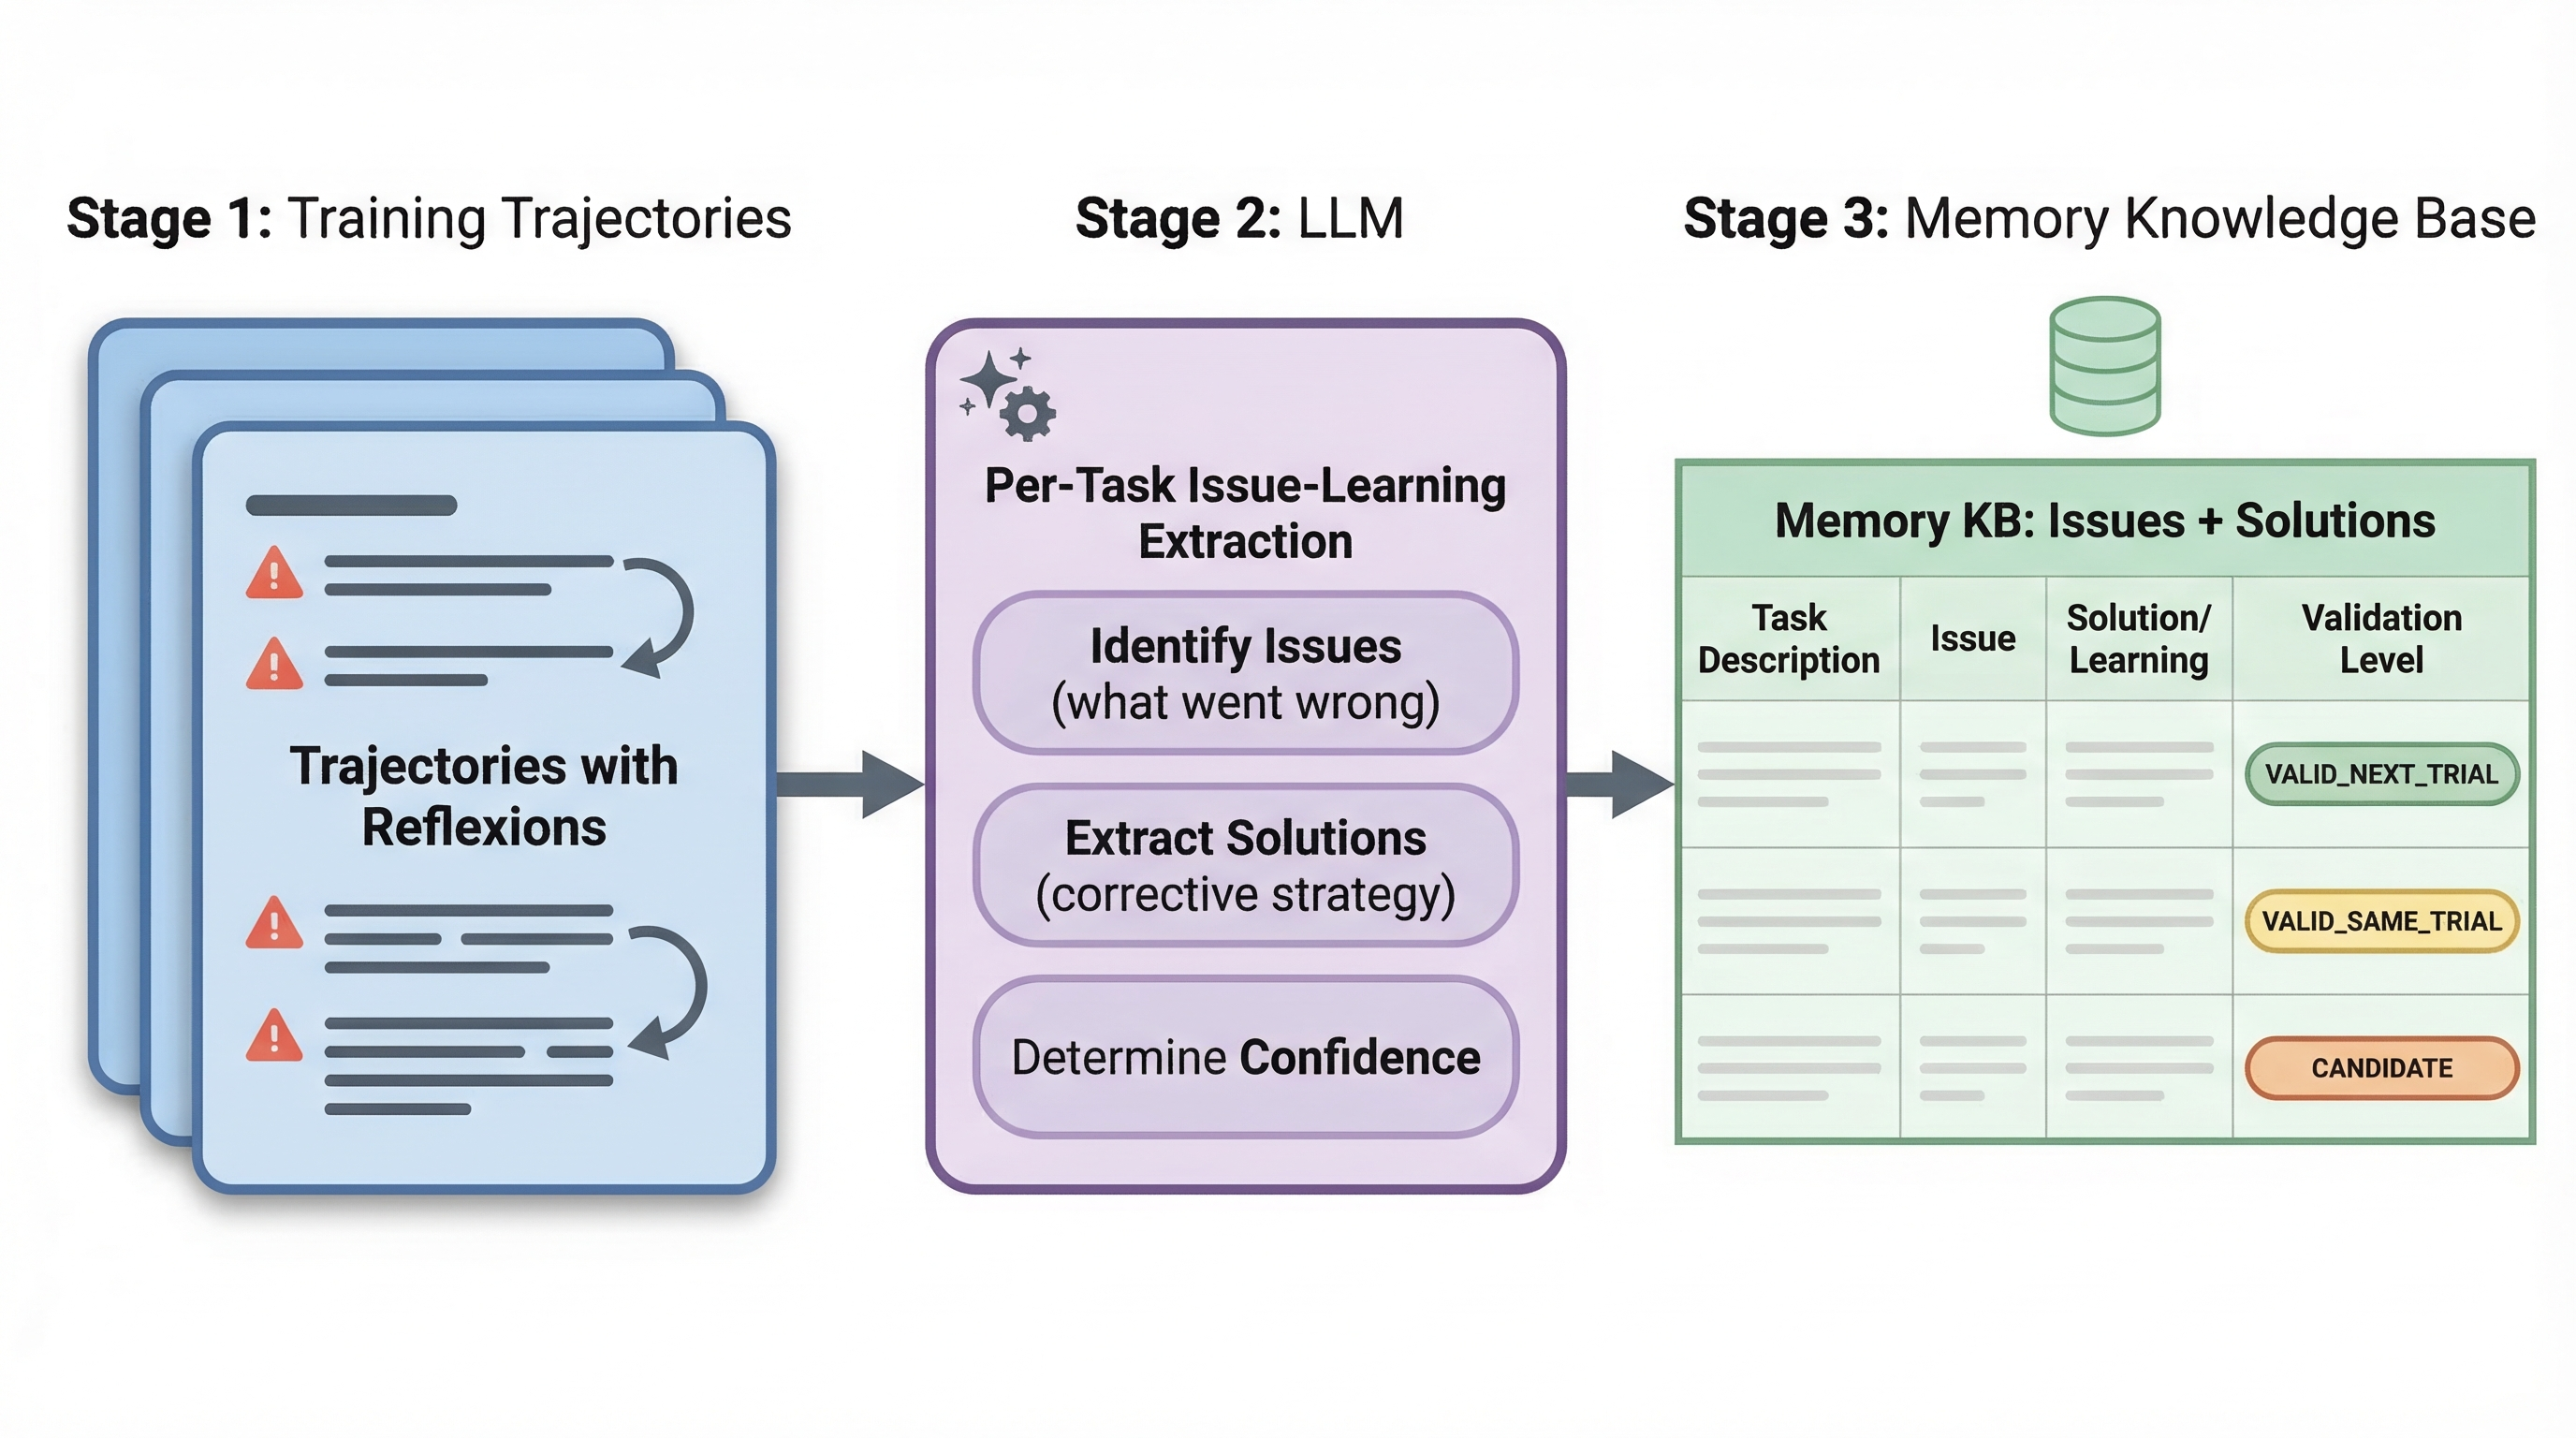
\includegraphics[width=\textwidth]{figures/section1_kb_generation.png}
    \caption{Offline KB construction from training trajectories.}
    \label{fig:kb-generation}
\end{subfigure}
\hfill
\begin{subfigure}[t]{0.48\textwidth}
    \centering
    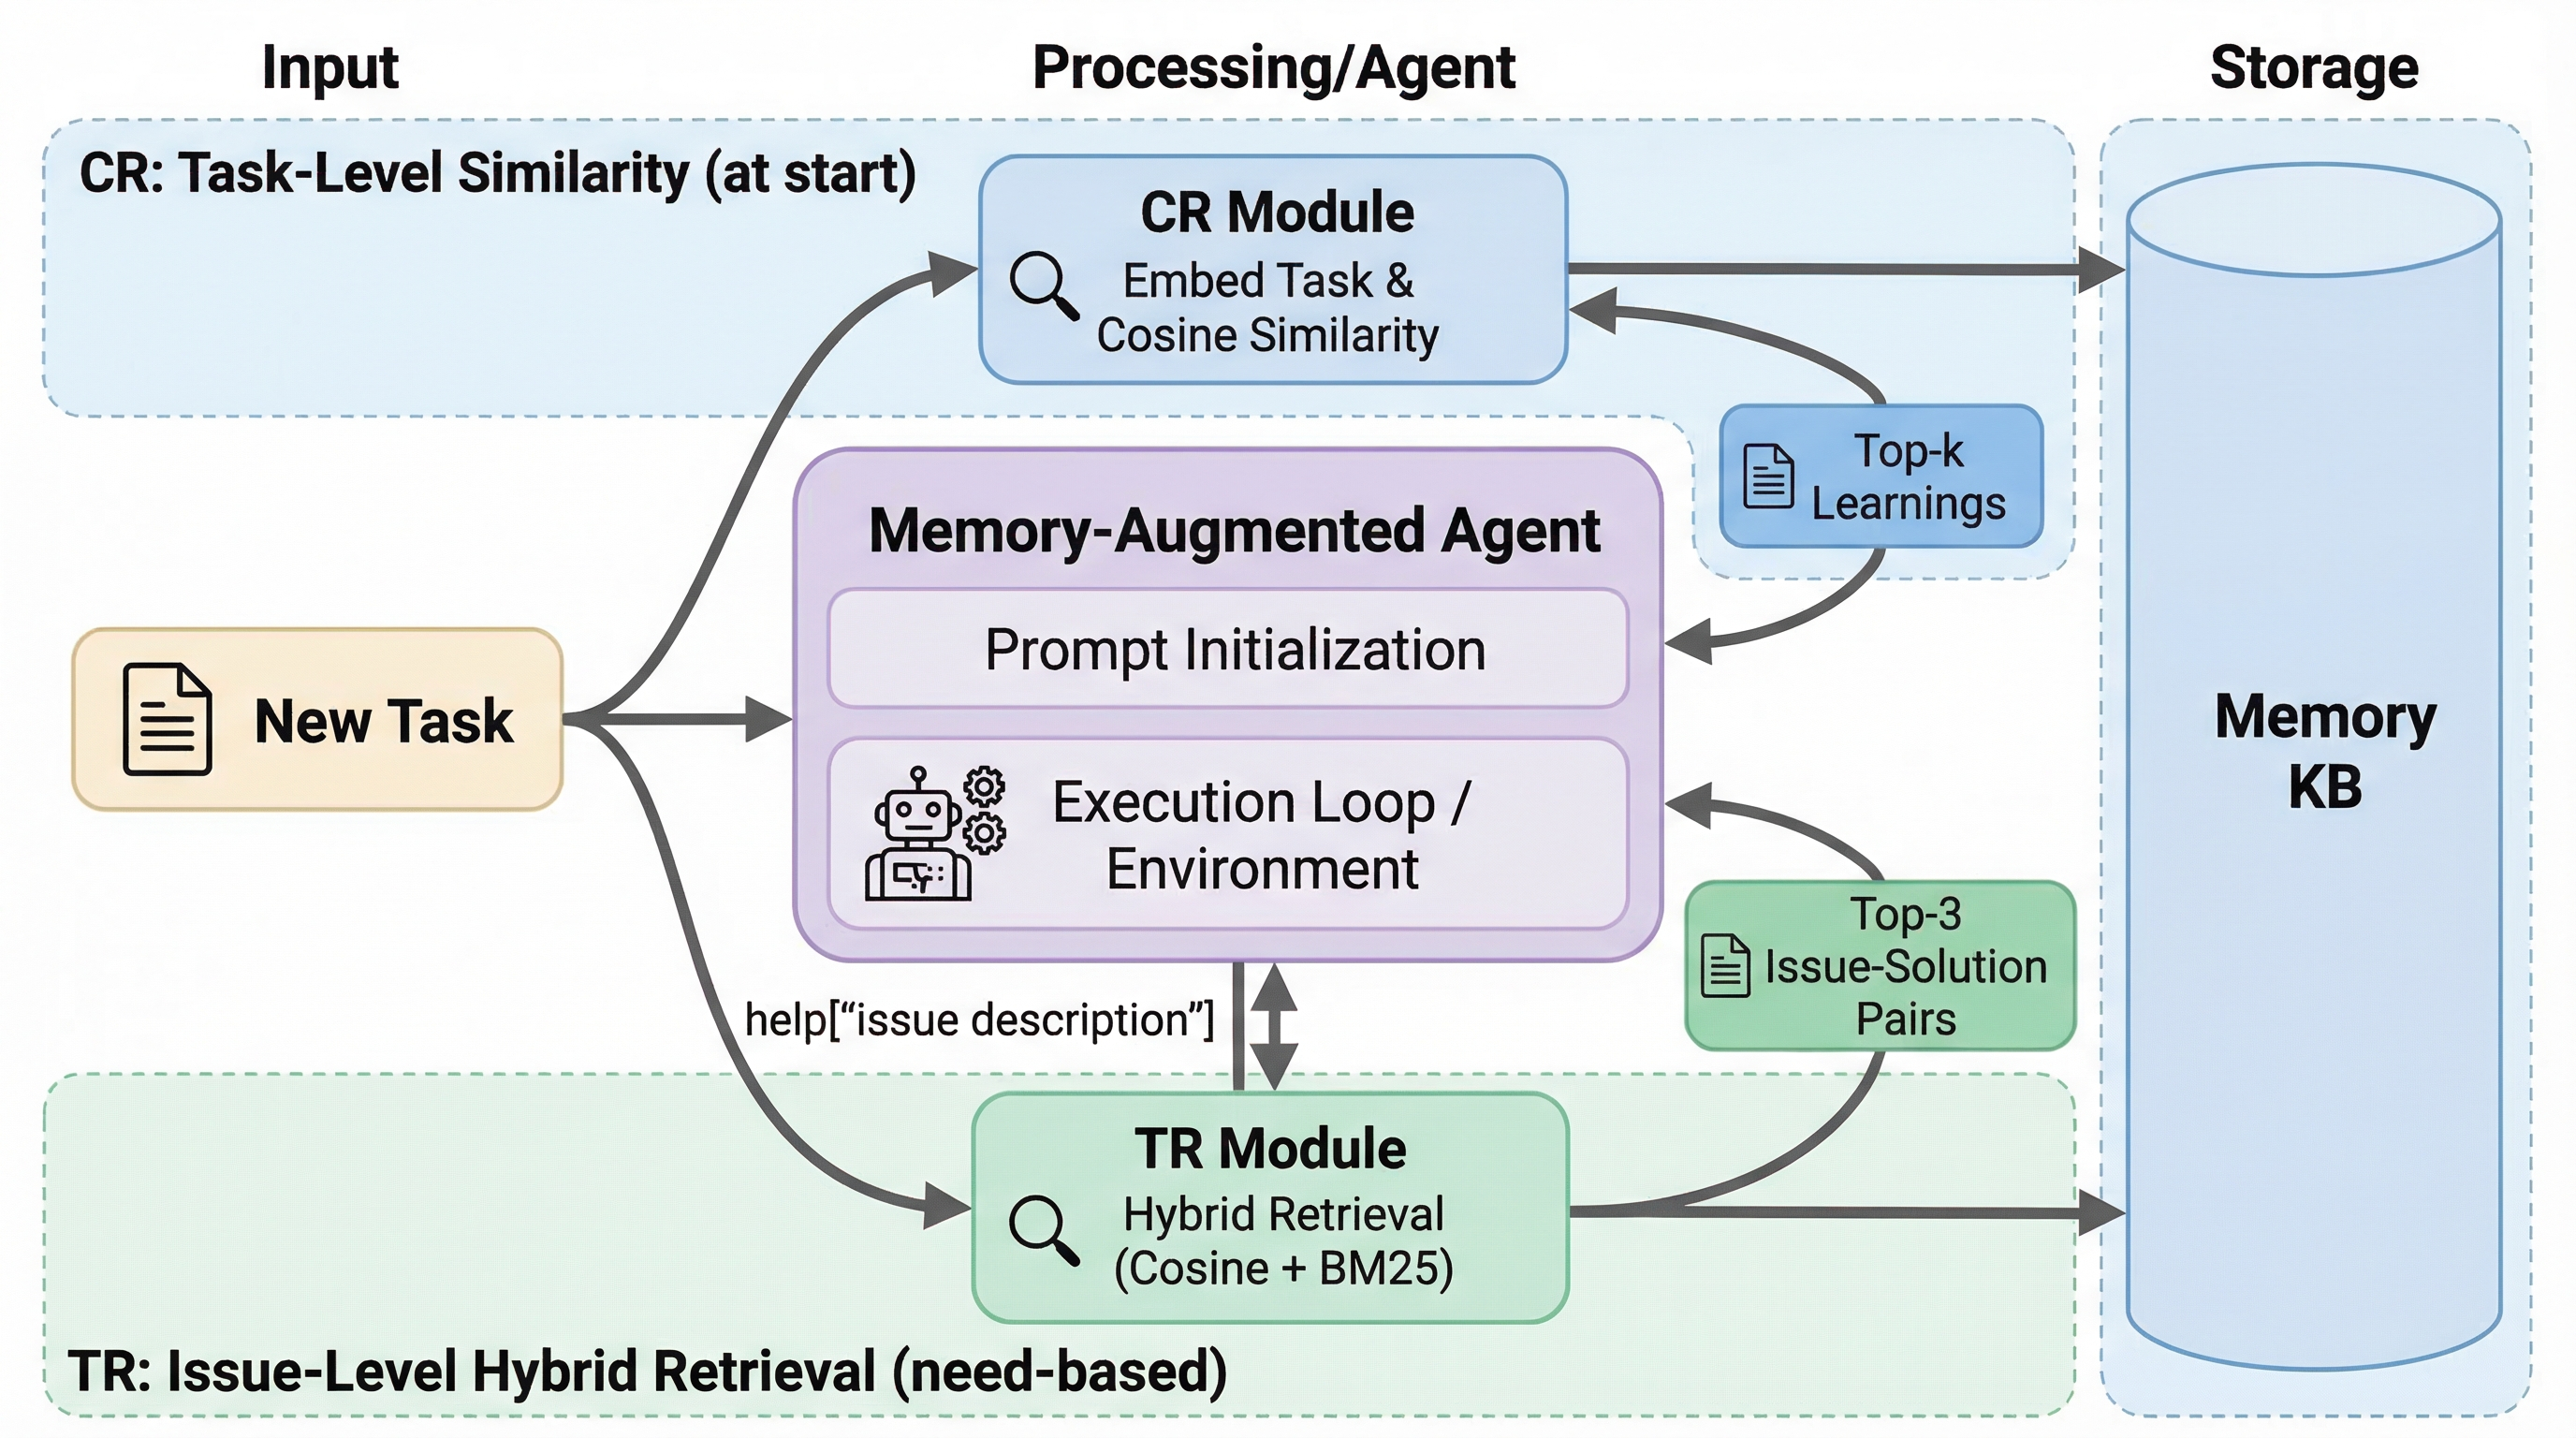
\includegraphics[width=\textwidth]{figures/section2_cr_tr_inference.png}
    \caption{Inference-time retrieval via CR and TR.}
    \label{fig:cr-tr-inference}
\end{subfigure}
\caption{Overview of the episodic memory framework. (a)~Training trajectories with reflexions are processed by an LLM to extract per-task issue--learning pairs with validation levels. (b)~Context Retrieval (CR) provides task-level learnings at the start; Tool Retrieval (TR) provides issue-level solutions on demand during execution.}
\label{fig:system-overview}
\end{figure*}

% ---- 3.3.1 ----
\subsubsection{Knowledge Base Construction}
\label{sec:kb-construction}

The knowledge base is constructed offline from training trajectories using LLM-based extraction. For each task, we extract \emph{issue--learning pairs}: structured records associating a mistake with its successful correction. Each entry includes task metadata, the issue--learning texts, a validation level reflecting downstream outcome (\textsc{Valid\_Next\_Trial}, \textsc{Valid\_Same\_Trial}, or \textsc{Candidate}), and provenance information. Final retrieval uses \textsc{Valid\_Next\_Trial} entries. We assign scalar validation weights $\omega$ to each level: $\omega_{\text{next}} = 1.0$, $\omega_{\text{same}} = 0.9$, $\omega_{\text{cand}} = 0.6$, used by both retrieval mechanisms to prioritize high-confidence learnings in the general algorithm. Full schema details are in Appendix~\ref{app:kb-schema}.

% ---- 3.3.2 ----
\subsubsection{Context Retrieval (CR)}
\label{sec:context-retrieval}

CR operates proactively: before the agent acts, it retrieves relevant past learnings based on embedding similarity (using \texttt{gemini-embedding-001}) between the new task description and historical tasks. The top-$k$ ($k{=}5$) most similar tasks are identified, their associated learnings are pooled and scored by:
\begin{equation}
    \text{Score}_{\text{CR}}(\ell) = \text{sim}(\mathbf{v}_q, \mathbf{v}_{t(\ell)}) \times \omega_{\ell}
\label{eq:cr-score}
\end{equation}
where $\text{sim}$ is cosine similarity and $\omega_{\ell}$ is the validation weight.

\paragraph{Dynamic context sizing.}
Rather than retrieving a fixed number of learnings, CR adapts the context window to neighborhood complexity. Let $L_{\max}$ denote the maximum learning count among the top-$k$ tasks. The retrieval quota is:
\begin{equation}
    N_{\text{pick}} = \min\!\left(\left\lceil \alpha \cdot L_{\max} \right\rceil,\; p\right)
\end{equation}
where $\alpha = 1.5$ is a scaling factor and $p \in [5, 25]$ is a tunable cap. The top-scored learnings are formatted as issue--learning pairs and prepended to the agent's prompt. The full procedure is given in Algorithm~\ref{alg:context-retrieval} (Appendix~\ref{app:algorithms}).

% ---- 3.3.3 ----
\subsubsection{Tool Retrieval (TR)}
\label{sec:tool-retrieval}

TR provides on-demand retrieval exposed as an action \texttt{help["issue"]}. It uses hybrid dense--sparse retrieval: cosine similarity over issue embeddings captures semantic matches, while BM25~\cite{robertson2009bm25} over concatenated fields captures lexical matches. The candidate pool is the union of the top-100 results from each strategy. Scores are normalized to $[0, 1]$ and fused:
\begin{equation}
    \text{Score}_{\text{TR}}(e) = \left(0.7 \cdot \text{cos}_{\text{norm}} + 0.3 \cdot \text{BM25}_{\text{norm}}\right) \times \omega_{e}
\label{eq:tr-score}
\end{equation}
The top-$k$ ($k{=}3$) results are returned as issue--solution pairs. The full procedure is given in Algorithm~\ref{alg:tool-retrieval} (Appendix~\ref{app:algorithms}).

% ---- 3.3.4 ----
\subsubsection{Hard Negative Control}
\label{sec:hard-neg}

To verify that gains stem from retrieval \emph{relevance} rather than additional prompt context, we introduce a hard negative control that inverts the selection criterion: CR retrieves the \emph{least} similar tasks and TR selects from the bottom of each retrieval strategy, producing prompts with the same number of learnings but from maximally irrelevant tasks.

% ----------------------------------------------------------------------------
\subsection{Reflexion for KB Construction}
\label{sec:reflexion}

We use Reflexion~\cite{shinn2023reflexion}, an iterative self-correction framework, to generate training trajectories for the trials7 knowledge bases. Unlike inference-time CR and TR, Reflexion is intra-task: it retries the same task with accumulated self-critiques. Our final held-out comparisons evaluate single-trial ReAct variants with and without retrieved cross-task memory.


% ============================================================================
% 4. EXPERIMENTAL SETUP
% ============================================================================
\section{Experimental Setup}
\label{sec:experimental-setup}

All agent reasoning uses Gemini 2.5 Flash, and all retrieval embeddings use Google's \texttt{text-embedding-004}, held constant across experiments.

\paragraph{Tasks and splits.}
For ALFWorld, the knowledge base is constructed from \emph{alfworld-mini}, a curated subset of 120 training games (20 per task type). We evaluate on the standard validation-seen (140 tasks) and validation-unseen (134 tasks) splits. For WebShop, we evaluate on development (200 tasks) and held-out test (200 tasks) splits, with the knowledge base extracted from separate training tasks. Full dataset details are in Appendix~\ref{app:experimental-details}.

\paragraph{Framework variants.}
We evaluate six variants per environment: ReAct (baseline), ReAct + Reflexion (up to 7 trials), ReAct + CR, ReAct + TR, ReAct + CR + TR, and a hard-negative ablation control. All memory variants execute a single trial per task.

\paragraph{Metrics.}
We report accuracy (binary success rate), average steps per trial and per task (capturing Reflexion's cumulative retry cost), and gain from the ReAct baseline in percentage points. Full metric definitions are in Appendix~\ref{app:experimental-details}.


% ============================================================================
% 5. RESULTS
% ============================================================================
\section{Results}
\label{sec:results}

\begin{table*}[t]
\centering
\caption{Final held-out Stage C results using train-only trials7 KBs, Gemini Flash, Gemini embeddings, \texttt{VALID\_NEXT\_TRIAL}, and \texttt{max\_learnings=5}. Values are mean $\pm$ std over three seeds.}
\label{tab:final-main-results}
\begin{tabular}{llrrrr}
\toprule
Environment & Framework & Tasks & Success (\%) & Score & $\Delta$ success (pp) \\
\midrule
ALFWorld & ReAct & 134 & 67.9 $\pm$ 0.0 & 0.679 $\pm$ 0.000 & \textemdash{} \\
ALFWorld & ReAct + CR & 134 & 63.9 $\pm$ 1.6 & 0.639 $\pm$ 0.016 & -4.0 $\pm$ 1.6 \\
ALFWorld & ReAct + TR & 134 & 75.4 $\pm$ 0.0 & 0.754 $\pm$ 0.000 & +7.5 $\pm$ 0.0 \\
ALFWorld & ReAct + CR + TR & 134 & \textbf{82.8 $\pm$ 0.0} & 0.828 $\pm$ 0.000 & +14.9 $\pm$ 0.0 \\
ALFWorld & Hard-neg CR + TR & 134 & 55.2 $\pm$ 0.7 & 0.552 $\pm$ 0.007 & -12.7 $\pm$ 0.7 \\
\midrule
SQL & ReAct & 200 & 91.5 $\pm$ 0.0 & 0.920 $\pm$ 0.000 & \textemdash{} \\
SQL & ReAct + CR & 200 & 88.5 $\pm$ 0.0 & 0.889 $\pm$ 0.001 & -3.0 $\pm$ 0.0 \\
SQL & ReAct + TR & 200 & 90.8 $\pm$ 0.3 & 0.917 $\pm$ 0.003 & -0.7 $\pm$ 0.3 \\
SQL & ReAct + CR + TR & 200 & \textbf{92.0 $\pm$ 0.0} & 0.922 $\pm$ 0.000 & +0.5 $\pm$ 0.0 \\
SQL & Hard-neg CR + TR & 200 & 89.5 $\pm$ 0.0 & 0.906 $\pm$ 0.000 & -2.0 $\pm$ 0.0 \\
\midrule
ScienceWorld & ReAct & 30 & \textbf{30.0 $\pm$ 8.8} & 0.214 $\pm$ 0.241 & \textemdash{} \\
ScienceWorld & ReAct + CR & 30 & 26.7 $\pm$ 3.3 & 0.171 $\pm$ 0.058 & -3.3 $\pm$ 12.0 \\
ScienceWorld & ReAct + TR & 30 & 26.7 $\pm$ 3.3 & 0.256 $\pm$ 0.086 & -3.3 $\pm$ 6.7 \\
ScienceWorld & ReAct + CR + TR & 30 & 27.8 $\pm$ 7.7 & 0.212 $\pm$ 0.134 & -2.2 $\pm$ 6.9 \\
ScienceWorld & Hard-neg CR + TR & 30 & 28.9 $\pm$ 6.9 & 0.260 $\pm$ 0.149 & -1.1 $\pm$ 15.4 \\
\bottomrule
\end{tabular}
\vspace{2pt}
{\footnotesize Score is average reward when logged; for ALFWorld ReAct, success rate is used because reward was not emitted in the final record.}
\end{table*}

\begin{table*}[t]
\centering
\caption{Final train-only KB inventory for the trials7 protocol. VNT = \texttt{VALID\_NEXT\_TRIAL}.}
\label{tab:final-kb-inventory}
\small
\resizebox{\textwidth}{!}{%
\begin{tabular}{@{}lp{0.20\linewidth}p{0.16\linewidth}cccp{0.22\linewidth}@{}}
\toprule
Environment & KB artifact & Coverage & Max trial & Memories & VNT & Audit note \\
\midrule
ALFWorld & \shortstack[l]{\texttt{alfworld\_train}\\\texttt{reflexion\_trials7}} & 115/120 observed train games & 7 & 373 & 101 & Train-only refs; no eval overlap; original 120-game manifest absent. \\
SQL & \shortstack[l]{\texttt{sql\_train\_reflexion}\\\texttt{trials7\_sanitized}} & 516/516 train tasks & 7 & 415 & 92 & Sanitized; no dev/test overlap; protocol memories quarantined. \\
ScienceWorld & \shortstack[l]{\texttt{scienceworld\_train}\\\texttt{reflexion\_trials7}\\\texttt{va80\_30cat}} & 30/30 categories, 30 variations & 7 & 129 & 34 & Train-only; 1 variation/category; failed extractions repaired. \\
\bottomrule
\end{tabular}
}
\end{table*}


\begin{figure*}[t]
\centering
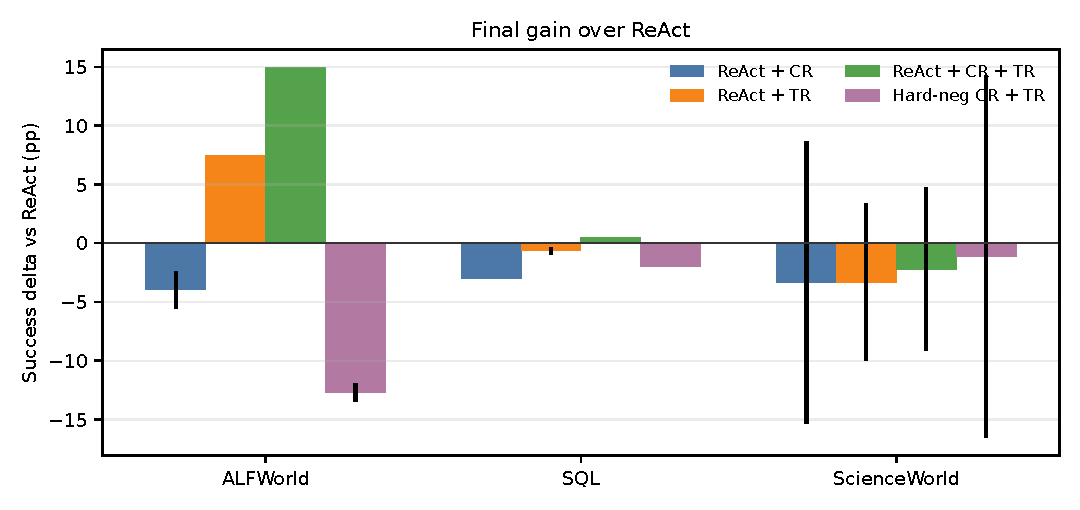
\includegraphics[width=\linewidth]{figures/final_gain_over_react.pdf}
\caption{Final success gain over ReAct for each memory variant. ALFWorld shows a clear positive CR+TR effect, SQL shows a narrow CR+TR effect, and ScienceWorld does not show a promoted positive memory result.}
\label{fig:final-gain-over-react}
\end{figure*}

\begin{figure}[t]
\centering
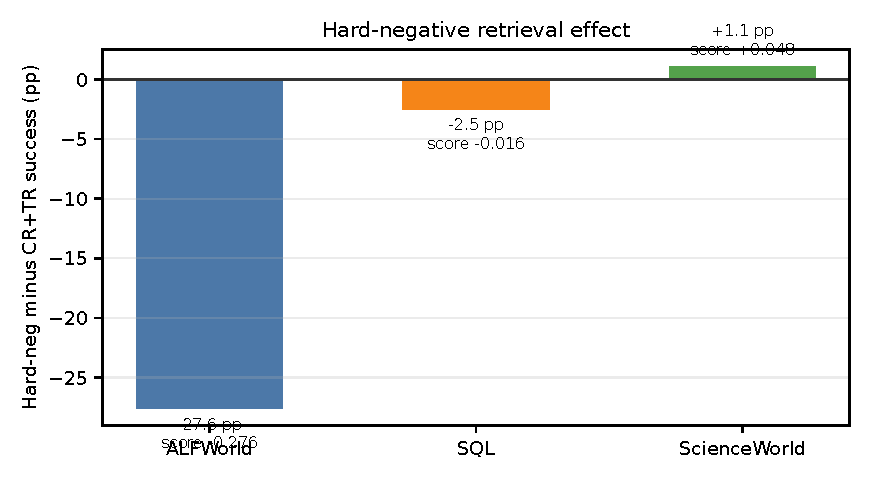
\includegraphics[width=\linewidth]{figures/final_hard_negative_effect.pdf}
\caption{Hard-negative effect in the final audits. The ALFWorld gap between CR+TR and hard-negative retrieval supports relevance as causal; the SQL and ScienceWorld gaps are smaller or unfavorable.}
\label{fig:final-hard-negative-effect}
\end{figure}

Table~\ref{tab:final-main-results} reports the final held-out Stage C results.
The headline is conditional: validated memory helps strongly in ALFWorld, weakly in SQL, and fails to promote ScienceWorld.

\subsection{ALFWorld: Positive Transfer}
\label{sec:results-alfworld}

ALFWorld is the clean positive case.
ReAct solves $67.9\%$ of the 134 validation-unseen tasks, while CR+TR solves $82.8\%$, a $+14.9$pp improvement.
TR alone is also positive ($75.4\%$, $+7.5$pp), while CR alone is negative ($63.9\%$, $-4.0$pp), showing that the two channels are useful but not automatically additive in isolation.
The combined channel is strongest, suggesting that proactive task-level context and on-demand issue-level retrieval can complement each other when the environment has reusable procedures.

The hard-negative control is decisive in ALFWorld.
Hard-negative CR+TR reaches only $55.2\%$, which is $27.6$pp below proper CR+TR and $12.7$pp below ReAct.
This rules against a simple ``extra context helps'' explanation: retrieved memory helps only when it is relevant to the task structure.

\subsection{SQL: Narrow Transfer}
\label{sec:results-sql}

SQL is a narrow-transfer diagnostic rather than a large positive result.
ReAct is already strong at $91.5\%$ success, leaving little headroom.
CR+TR improves to $92.0\%$, a small $+0.5$pp gain, but CR alone falls to $88.5\%$ and TR alone to $90.8\%$.
Hard-negative CR+TR reaches $89.5\%$, also below ReAct.

The SQL pattern indicates that some validated memories transfer, but the transfer radius is small.
Useful query repairs can be highly local to a schema, predicate, or join pattern.
This makes SQL evidence for conditional memory benefit: the best combined retrieval channel can help slightly, but individual channels and irrelevant retrievals can easily perturb a high-performing baseline.

\subsection{ScienceWorld: Diagnostic Negative Evidence}
\label{sec:results-scienceworld}

ScienceWorld should not be read as a positive transfer result.
In the final Stage C audit, ReAct is the best framework at $30.0\%$ success.
CR, TR, and CR+TR all fall below ReAct on mean success, with CR+TR at $27.8\%$.
Hard-negative CR+TR reaches $28.9\%$, matching or exceeding proper CR+TR on the headline metric.

This matters because the ScienceWorld final KB is clean but thin: it covers all 30 categories, yet only one train variation per category.
The later Phase 4.1 density gate tested whether increasing to three train variations per category would rescue the result.
It did not: same-run CR+TR underperformed ReAct on mean success and mean reward, and hard-negative retrieval matched or beat CR+TR on success in every seed.
We therefore use ScienceWorld as diagnostic evidence that memory density alone is insufficient when retrieval and validation signals do not align with reusable task structure.

\subsection{Usage, Cost, and Paired Deltas}
\label{sec:usage-deltas}

\begin{table*}[t]
\centering
\caption{Final memory usage and trajectory cost summaries from raw trajectories. Values are mean $\pm$ std over seeds.}
\label{tab:final-memory-usage}
\begin{tabular}{llrrrrr}
\toprule
Environment & Framework & Context tasks & Retrieved/task & Help calls & Help/task & Steps/task \\
\midrule
ALFWorld & ReAct & 0.0 $\pm$ 0.0 & 0.00 $\pm$ 0.00 & 0.0 $\pm$ 0.0 & 0.00 $\pm$ 0.00 & 21.00 $\pm$ 0.11 \\
ALFWorld & ReAct + CR & 132.0 $\pm$ 0.0 & 4.05 $\pm$ 0.00 & 0.0 $\pm$ 0.0 & 0.00 $\pm$ 0.00 & 28.56 $\pm$ 0.26 \\
ALFWorld & ReAct + TR & 0.0 $\pm$ 0.0 & 0.00 $\pm$ 0.00 & 302.3 $\pm$ 0.6 & 2.26 $\pm$ 0.00 & 27.69 $\pm$ 0.01 \\
ALFWorld & ReAct + CR + TR & 132.0 $\pm$ 0.0 & 4.05 $\pm$ 0.00 & 206.0 $\pm$ 0.0 & 1.54 $\pm$ 0.00 & 26.38 $\pm$ 0.01 \\
ALFWorld & Hard-neg CR + TR & 134.0 $\pm$ 0.0 & 4.67 $\pm$ 0.00 & 360.3 $\pm$ 6.4 & 2.69 $\pm$ 0.05 & 34.72 $\pm$ 0.08 \\
\midrule
SQL & ReAct & 0.0 $\pm$ 0.0 & 0.00 $\pm$ 0.00 & 0.0 $\pm$ 0.0 & 0.00 $\pm$ 0.00 & 8.67 $\pm$ 0.00 \\
SQL & ReAct + CR & 178.0 $\pm$ 0.0 & 2.05 $\pm$ 0.00 & 0.0 $\pm$ 0.0 & 0.00 $\pm$ 0.00 & 8.94 $\pm$ 0.00 \\
SQL & ReAct + TR & 0.0 $\pm$ 0.0 & 0.00 $\pm$ 0.00 & 23.0 $\pm$ 0.0 & 0.12 $\pm$ 0.00 & 9.23 $\pm$ 0.00 \\
SQL & ReAct + CR + TR & 178.0 $\pm$ 0.0 & 2.05 $\pm$ 0.00 & 20.0 $\pm$ 0.0 & 0.10 $\pm$ 0.00 & 9.11 $\pm$ 0.01 \\
SQL & Hard-neg CR + TR & 171.7 $\pm$ 0.6 & 1.68 $\pm$ 0.01 & 24.0 $\pm$ 0.0 & 0.12 $\pm$ 0.00 & 9.03 $\pm$ 0.00 \\
\midrule
ScienceWorld & ReAct & 0.0 $\pm$ 0.0 & 0.00 $\pm$ 0.00 & 0.0 $\pm$ 0.0 & 0.00 $\pm$ 0.00 & 30.96 $\pm$ 1.67 \\
ScienceWorld & ReAct + CR & 30.0 $\pm$ 0.0 & 4.40 $\pm$ 0.00 & 0.0 $\pm$ 0.0 & 0.00 $\pm$ 0.00 & 30.48 $\pm$ 1.24 \\
ScienceWorld & ReAct + TR & 0.0 $\pm$ 0.0 & 0.00 $\pm$ 0.00 & 37.3 $\pm$ 6.4 & 1.24 $\pm$ 0.21 & 34.19 $\pm$ 2.13 \\
ScienceWorld & ReAct + CR + TR & 30.0 $\pm$ 0.0 & 4.40 $\pm$ 0.00 & 20.7 $\pm$ 3.8 & 0.69 $\pm$ 0.13 & 31.23 $\pm$ 1.99 \\
ScienceWorld & Hard-neg CR + TR & 30.0 $\pm$ 0.0 & 4.17 $\pm$ 0.00 & 31.3 $\pm$ 2.1 & 1.04 $\pm$ 0.07 & 33.08 $\pm$ 0.37 \\
\bottomrule
\end{tabular}
\end{table*}

\begin{table*}[t]
\centering
\caption{Paired task-level deltas against ReAct on the final held-out Stage C runs. Values are mean $\pm$ std over seeds.}
\label{tab:final-paired-deltas}
\resizebox{\textwidth}{!}{%
\begin{tabular}{llrrrrr}
\toprule
Environment & Framework & Common tasks & $\Delta$ success (pp) & $\Delta$ score & Improved & Regressed \\
\midrule
ALFWorld & ReAct + CR & 134 $\pm$ 0 & -4.0 $\pm$ 1.6 & \textemdash{} & 20.3 $\pm$ 1.5 & 25.7 $\pm$ 0.6 \\
ALFWorld & ReAct + TR & 134 $\pm$ 0 & +7.5 $\pm$ 0.0 & \textemdash{} & 27.0 $\pm$ 0.0 & 17.0 $\pm$ 0.0 \\
ALFWorld & ReAct + CR + TR & 134 $\pm$ 0 & +14.9 $\pm$ 0.0 & \textemdash{} & 33.0 $\pm$ 0.0 & 13.0 $\pm$ 0.0 \\
ALFWorld & Hard-neg CR + TR & 134 $\pm$ 0 & -12.7 $\pm$ 0.7 & \textemdash{} & 18.7 $\pm$ 0.6 & 35.7 $\pm$ 0.6 \\
\midrule
SQL & ReAct + CR & 200 $\pm$ 0 & -3.0 $\pm$ 0.0 & -0.031 $\pm$ 0.001 & 2.0 $\pm$ 0.0 & 8.0 $\pm$ 0.0 \\
SQL & ReAct + TR & 200 $\pm$ 0 & -0.7 $\pm$ 0.3 & -0.003 $\pm$ 0.003 & 2.0 $\pm$ 0.0 & 3.3 $\pm$ 0.6 \\
SQL & ReAct + CR + TR & 200 $\pm$ 0 & +0.5 $\pm$ 0.0 & 0.002 $\pm$ 0.000 & 3.0 $\pm$ 0.0 & 2.0 $\pm$ 0.0 \\
SQL & Hard-neg CR + TR & 200 $\pm$ 0 & -2.0 $\pm$ 0.0 & -0.014 $\pm$ 0.000 & 2.0 $\pm$ 0.0 & 6.0 $\pm$ 0.0 \\
\midrule
ScienceWorld & ReAct + CR & 30 $\pm$ 0 & -3.3 $\pm$ 12.0 & -0.043 $\pm$ 0.284 & 2.7 $\pm$ 1.2 & 3.7 $\pm$ 2.5 \\
ScienceWorld & ReAct + TR & 30 $\pm$ 0 & -3.3 $\pm$ 6.7 & 0.042 $\pm$ 0.240 & 3.0 $\pm$ 1.0 & 4.0 $\pm$ 1.0 \\
ScienceWorld & ReAct + CR + TR & 30 $\pm$ 0 & -2.2 $\pm$ 6.9 & -0.002 $\pm$ 0.148 & 2.0 $\pm$ 1.0 & 2.7 $\pm$ 1.2 \\
ScienceWorld & Hard-neg CR + TR & 30 $\pm$ 0 & -1.1 $\pm$ 15.4 & 0.046 $\pm$ 0.354 & 4.3 $\pm$ 1.5 & 4.7 $\pm$ 3.2 \\
\bottomrule
\end{tabular}
}
\end{table*}


\begin{figure*}[t]
\centering
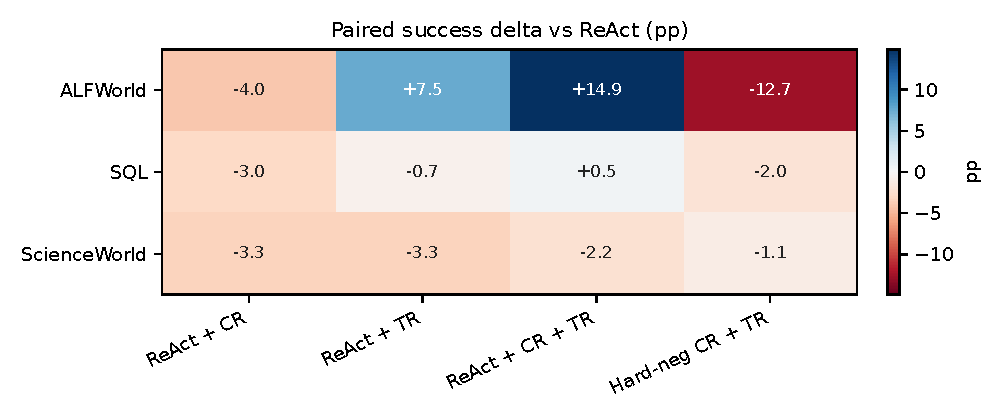
\includegraphics[width=\linewidth]{figures/final_paired_delta_heatmap.pdf}
\caption{Paired task-level deltas against ReAct. Positive and negative cells expose where memory helps, regresses, or remains neutral under matched task comparisons.}
\label{fig:final-paired-delta-heatmap}
\end{figure*}

\begin{figure}[t]
\centering
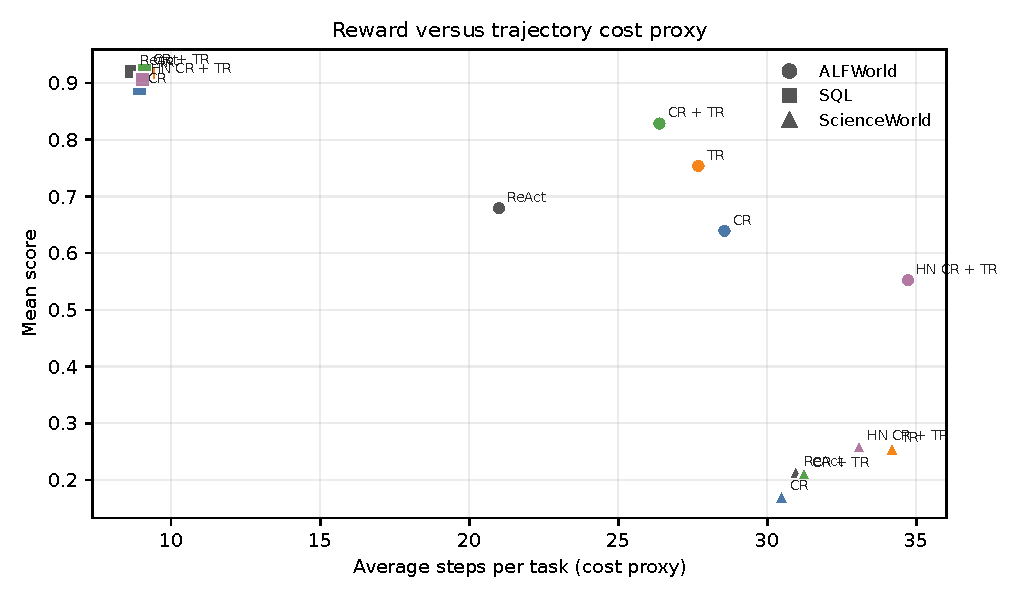
\includegraphics[width=\linewidth]{figures/final_reward_vs_cost.pdf}
\caption{Final score versus trajectory cost, using average steps per task as a cost proxy because provider dollar cost is unavailable in the final raw logs.}
\label{fig:final-reward-vs-cost}
\end{figure}

Table~\ref{tab:final-memory-usage} shows that retrieval was active in the memory variants and that trajectory cost changes differ by environment.
ALFWorld CR+TR uses both context memories and help calls while remaining far below the hard-negative variant in steps per task.
SQL retrieval is sparse, especially for TR, consistent with its narrow-transfer character.
ScienceWorld retrieval occurs reliably, but usage does not translate into better success.

Table~\ref{tab:final-paired-deltas} and Figure~\ref{fig:final-paired-delta-heatmap} sharpen the same picture at the task level.
ALFWorld CR+TR improves many more tasks than it regresses.
SQL CR+TR has only a small favorable imbalance.
ScienceWorld has unstable paired deltas with no promoted CR+TR advantage.


% ============================================================================
% 6. ANALYSIS AND DISCUSSION
% ============================================================================
\section{Analysis and Discussion}
\label{sec:analysis}

We trace the divergence between environments to three structural properties and synthesize them into a diagnostic framework.

% ----------------------------------------------------------------------------
\subsection{Task Compositionality}
\label{sec:compositionality}

ALFWorld tasks decompose into shared sub-goal phases (\textsc{Search} $\rightarrow$ \textsc{Acquire} $\rightarrow$ \textsc{Transform} $\rightarrow$ \textsc{Place}) that recur across task types, so a modest set of phase-specific learnings covers a combinatorially large task space. WebShop tasks are monolithic: each targets a unique product through a unique catalog path with no shared sub-task decomposition. This explains why CR yields $+15.7$pp on ALFWorld but $-29$pp on WebShop---and why the hard-negative paradox emerges: in WebShop, obviously irrelevant retrievals cause less harm than plausible-looking but non-transferable ones.

\paragraph{Principle.} Episodic memory is most effective when tasks share compositional sub-task structure.

% ----------------------------------------------------------------------------
\subsection{Action Space Regularity}
\label{sec:action-space}

ALFWorld's fixed grammar of ${\sim}$15 verb templates ensures that learned action sequences generalize across tasks. WebShop's action space is syntactically simple but combinatorially vast: free-form search queries and dynamically generated page elements mean that specific navigation paths never recur. TR's issue-level guidance accordingly helps in ALFWorld ($+8.2$pp unseen) but hurts in WebShop ($-21.5$pp).

\paragraph{Principle.} Episodic memory is most effective when the action space is constrained and regular.

% ----------------------------------------------------------------------------
\subsection{Learning Transfer Radius}
\label{sec:transfer-radius}

We define the \emph{learning transfer radius} as the number of distinct future tasks that benefit from a single learned experience. In ALFWorld, a learning like ``open the container before taking an object'' applies to dozens of tasks across multiple types (high radius). In WebShop, each learning is tied to a unique product (radius near zero). The empirical signature is visible in ALFWorld's stronger unseen-split gains ($+19.4$pp vs.\ $+16.4$pp on seen), indicating effective cross-task generalization.

\paragraph{Principle.} Episodic memory is most effective when the learning transfer radius is high.

% ----------------------------------------------------------------------------
\subsection{Efficiency--Accuracy Trade-off}
\label{sec:efficiency}

Figure~\ref{fig:accuracy-cost} plots accuracy against computational cost (steps per task) on held-out splits, revealing a key practical distinction. On ALFWorld, CR+TR occupies an efficient frontier: it achieves near-Reflexion accuracy ($+19.4$pp vs.\ $+21.6$pp) at roughly one-third the step cost (${\sim}$23 vs.\ ${\sim}$79 steps/task), making it the preferred choice when compute budgets are constrained. On WebShop, memory variants shift the agent into a strictly dominated region---accuracy degrades without any compensating reduction in cost. Reflexion improves accuracy in both environments but consistently incurs 3--4$\times$ the baseline step cost, highlighting the expense of iterative self-correction. This trade-off reinforces the environment-dependence of memory: when the three structural properties favor transfer, episodic memory provides a low-cost path to high accuracy; when they do not, the same mechanism wastes computation while actively degrading performance.

\subsection{Diagnostic Framework}
\label{sec:framework}

Table~\ref{tab:framework} summarizes how the two environments differ along these dimensions.

\begin{table}[t]
\centering
\small
\caption{Diagnostic framework for episodic memory effectiveness. Effect sizes relative to ReAct baseline (seen/unseen for ALFWorld, dev/test for WebShop).}
\label{tab:framework}
\resizebox{\columnwidth}{!}{%
\begin{tabular}{lcc}
\toprule
\textbf{Property} & \textbf{ALFWorld} & \textbf{WebShop} \\
\midrule
Task Compositionality & High (shared sub-goals) & Low (unique products) \\
Action Space Regularity & High (fixed, ${\sim}$15 verbs) & Low (free-form) \\
Learning Transfer Radius & High (1 $\rightarrow$ many tasks) & Near-zero \\
\midrule
Memory Effect (CR+TR) & $+16.4$/$+19.4$pp & $-30.5$/$-27.5$pp \\
Hard-neg Effect$^*$ & $-5.7$/$-17.2$pp & $-12.5$/$-15.0$pp \\
\bottomrule
\end{tabular}%
}
\vspace{2pt}

{\footnotesize $^*$Hard-neg \emph{outperforms} proper retrieval on WebShop ($-12.5$ vs.\ $-30.5$pp), indicating semantic similarity is counterproductive when transfer radius is near zero.}
\end{table}

When all three properties favor transfer, memory provides substantial gains; when they do not, retrieved experiences actively mislead the agent. Before deploying a memory system, practitioners should assess their target environment along these dimensions: task compositionality, action space regularity, and learning transfer radius. When these properties are unfavorable, alternatives such as intra-task self-correction or memory systems with explicit gating mechanisms may be more appropriate.


% ============================================================================
% 7. LIMITATIONS
% ============================================================================
\section{Limitations}
\label{sec:limitations}

All final evaluations use one base LLM, Gemini 2.5 Flash.
Different models may be more or less sensitive to retrieved memories, especially in narrow-transfer settings such as SQL or in procedural domains such as ScienceWorld.

The final evidence is intentionally restricted to audited runs.
ALFWorld, SQL, and ScienceWorld are the only headline environments in the final tables.
Older exploratory runs are preserved for provenance but are not used as final evidence here.
This makes the claims cleaner, but it also means the transfer-radius framework should be treated as a diagnostic hypothesis requiring broader validation.

The knowledge bases are train-only, but they differ in density and provenance.
The ALFWorld trials7 KB has no evaluation overlap after quarantine, but the exact legacy 120-game train manifest is absent and the audit observes 115 unique train trajectory task IDs.
The ScienceWorld final KB covers all 30 categories with only one train variation per category; the later 3-var density gate did not promote ScienceWorld, but a future method with better validation or retrieval alignment could change that result.

Finally, we do not report provider dollar cost because it is unavailable in the final raw logs.
Cost figures use average steps per task as a trajectory-cost proxy.
We also lack a final retrieval-budget ablation, so this paper does not determine whether different CR/TR budgets would improve the mixed or negative cases.


% ============================================================================
% 8. CONCLUSION
% ============================================================================
\section{Conclusion}
\label{sec:conclusion}

This work provides evidence that episodic memory is not a universal enhancement for LLM-based agents. Through a controlled study applying an identical memory system to ALFWorld and WebShop, we observe that the same retrieval mechanisms produce a ${\sim}47$pp swing in effect: up to $+19.4$pp improvement versus $-30.5$pp degradation. Our hard-negative ablation reveals that in the low-transfer environment we studied, irrelevant memories caused \emph{less} harm than semantically ``relevant'' ones, suggesting confident misdirection rather than noise injection as the failure mode — at least under these experimental conditions.

We attribute this divergence to three structural properties (task compositionality, action space regularity, and learning transfer radius) and contribute a diagnostic framework offering practitioners tentative criteria for anticipating when episodic memory may help or hurt. Because these criteria are grounded in two environments with a single base model, they should be treated as hypotheses to test rather than universal rules. Future directions include adaptive memory gating that suppresses retrieval when transfer confidence is low, validation on additional domains and models, and memory filtering strategies that assess transferability before injecting retrieved content.

\paragraph{AI Disclosure.}
AI writing assistants were used to help draft and edit portions of this manuscript. All scientific content, experimental design, and analysis were conducted by the authors.


% ============================================================================
% REFERENCES
% ============================================================================
\bibliography{references}

% ============================================================================
% APPENDIX
% ============================================================================
\appendix

\section*{Appendix}

\section{Retrieval Algorithms}
\label{app:algorithms}

\begin{algorithm}[h]
\caption{Context Retrieval from Knowledge Base}
\label{alg:context-retrieval}
\begin{algorithmic}[1]
\REQUIRE Task description $q$; knowledge base $\mathcal{K}$; neighbor count $k{=}5$; scaling factor $\alpha{=}1.5$; cap $p \in [5, 25]$; validation weights $W$
\ENSURE Selected learnings $C$

\STATE $\mathbf{v}_q \leftarrow \textsc{Embed}(q)$
\STATE $\mathcal{T}_{\text{top}} \leftarrow \text{Top-}k \text{ tasks in } \mathcal{K} \text{ by } \text{sim}(\mathbf{v}_q, \mathbf{v}_t)$ \COMMENT{filter exact matches}
\STATE $L_{\max} \leftarrow \max_{t \in \mathcal{T}_{\text{top}}} \textsc{LearningCount}(t)$
\STATE $N_{\text{pick}} \leftarrow \min(\lceil \alpha \cdot L_{\max} \rceil, \; p)$
\STATE $\mathcal{L}_{\text{pool}} \leftarrow \emptyset$
\FOR{each $(t, s_t) \in \mathcal{T}_{\text{top}}$}
    \FOR{each learning $\ell \in \textsc{GetLearnings}(t)$}
        \STATE $\text{score}(\ell) \leftarrow s_t \times W[\ell.\text{valid\_level}]$
        \STATE $\mathcal{L}_{\text{pool}} \leftarrow \mathcal{L}_{\text{pool}} \cup \{(\ell, \text{score}(\ell))\}$
    \ENDFOR
\ENDFOR
\STATE Sort $\mathcal{L}_{\text{pool}}$ by score descending; deduplicate by learning text
\STATE $C \leftarrow$ first $N_{\text{pick}}$ elements of $\mathcal{L}_{\text{pool}}$
\RETURN $C$
\end{algorithmic}
\end{algorithm}

\begin{algorithm}[h]
\caption{Hybrid Tool Retrieval}
\label{alg:tool-retrieval}
\begin{algorithmic}[1]
\REQUIRE Issue description $I_q$; knowledge base $\mathcal{K}$; result count $k{=}3$; dense weight $\alpha{=}0.7$; sparse weight $\beta{=}0.3$; validation weights $W$
\ENSURE Top-$k$ issue--learning pairs

\STATE $q' \leftarrow \textsc{Clean}(I_q)$ \COMMENT{remove digits, normalize}
\STATE $\mathbf{v}_q \leftarrow \textsc{Embed}(q')$
\STATE $\mathbf{s}_{\cos} \leftarrow \textsc{CosineSim}(\mathbf{v}_q, \mathcal{K}.\text{issue\_embeddings})$
\STATE $\mathbf{s}_{\text{bm25}} \leftarrow \textsc{BM25}(q', \mathcal{K}.\text{index})$
\STATE $\mathcal{C} \leftarrow \text{Top}(\mathbf{s}_{\cos}, 100) \cup \text{Top}(\mathbf{s}_{\text{bm25}}, 100)$ \COMMENT{candidate pool}
\FOR{each $i \in \mathcal{C}$}
    \STATE $c_i \leftarrow \text{clamp}(\mathbf{s}_{\cos}[i], 0, 1)$
    \STATE $b_i \leftarrow \textsc{MinMaxNorm}(\mathbf{s}_{\text{bm25}}[i], \mathcal{C})$
    \STATE $S_{\text{hybrid}} \leftarrow \alpha \cdot c_i + \beta \cdot b_i$
    \STATE $\text{score}(i) \leftarrow S_{\text{hybrid}} \times W[\mathcal{K}[i].\text{valid\_level}]$
\ENDFOR
\STATE Sort $\mathcal{C}$ by score descending
\RETURN first $k$ elements of $\mathcal{C}$
\end{algorithmic}
\end{algorithm}

\section{Knowledge Base Schema}
\label{app:kb-schema}

Each entry in the knowledge base is a structured record containing the following fields:

\begin{itemize}
    \item \textbf{Task metadata}: task description, object type, action verbs, goal phase (\textsc{Search}, \textsc{Acquire}, \textsc{Transform}, \textsc{Place}, or \textsc{Recover}).
    \item \textbf{Issue--learning pair}: \texttt{issue\_text} (the specific mistake encountered) and \texttt{learning\_text} (the successful correction).
    \item \textbf{Validation level}: a confidence label reflecting downstream outcome:
    \begin{itemize}
        \item \textsc{Valid\_Next\_Trial}: the learning was applied and led to success in a subsequent trial (highest confidence). Weight $\omega_{\text{next}} = 1.0$.
        \item \textsc{Valid\_Same\_Trial}: the learning is associated with success within the same trial. Weight $\omega_{\text{same}} = 0.9$.
        \item \textsc{Candidate}: the learning was generated but the task was not completed (lowest confidence). Weight $\omega_{\text{cand}} = 0.6$.
    \end{itemize}
    \item \textbf{Provenance}: references to the source task, trial number, and step range for both the issue and its resolution.
\end{itemize}

\section{Experimental Details}
\label{app:experimental-details}

\subsection{Dataset Statistics}

\paragraph{ALFWorld.}
The full ALFWorld dataset~\citep{shridhar2021alfworld} comprises 3{,}827 games split into a training set (3{,}553 games), a validation-seen set (140 games), and a validation-unseen set (134 games). For knowledge base construction, we use \emph{alfworld-mini}, a curated subset of 120 training games (20 per task type $\times$ 6 task types). We run Reflexion on this subset and extract approximately 400 issue--learning entries from the resulting trajectories using the pipeline described in Section~\ref{sec:kb-construction}. The validation splits are identical to those of the full ALFWorld dataset, ensuring direct comparability with prior work. No training games appear in the validation sets.

\paragraph{WebShop.}
We partition the WebShop environment~\citep{yao2022webshop} into a development split (200 tasks) and a held-out test split (200 tasks). The knowledge base is extracted from Reflexion training trajectories on a separate set of training tasks with no overlap with either evaluation split, yielding approximately 677 issue--learning entries.

\paragraph{SQL diagnostic gate.}
We include a paired SQL diagnostic gate of 50 tasks run with GPT-5.4 to probe transfer behavior in a formally regular action space. This gate is used as diagnostic evidence rather than as a full third benchmark. The paired run contains zero retrieved-help calls across memory variants and no environment-error matches in world logs, isolating memory and prompt effects from runner instability. Summary outputs are stored in the SQL transfer-radius experiment report directory.

\subsection{Framework Variants}

We evaluate six framework variants in each environment:
\begin{enumerate}
    \item \textbf{ReAct}: the base agent with no memory~\citep{yao2023react}, serving as the primary baseline.
    \item \textbf{ReAct + Reflexion}: the iterative self-correction baseline~\citep{shinn2023reflexion}, allowed up to 7 trials per task.
    \item \textbf{ReAct + CR}: base agent augmented with Context Retrieval only.
    \item \textbf{ReAct + TR}: base agent augmented with Tool Retrieval only.
    \item \textbf{ReAct + CR + TR}: base agent augmented with both retrieval mechanisms.
    \item \textbf{ReAct + hard-neg CR + TR}: ablation control that retrieves maximally \emph{irrelevant} entries via inverted retrieval (Section~\ref{sec:hard-neg}).
\end{enumerate}
All memory-augmented variants (CR, TR, CR+TR) execute a single trial per task, whereas Reflexion may execute up to 7 trials.

\subsection{Evaluation Metrics}

\paragraph{Task success.}
The fraction of tasks completed successfully, computed as a binary outcome per task. For WebShop, this is corrected strict success.

\paragraph{Average Steps per Trial.}
The mean number of thought--action--observation steps per individual trial attempt. For Reflexion, this reflects the average length of a single trial, irrespective of retry count.

\paragraph{Average Steps per Task.}
The mean total steps per task across all trials. For single-trial methods, this equals Steps/Trial. For Reflexion, this accumulates steps across all retry trials (up to 7), capturing the full computational cost.

\paragraph{Gain from ReAct.}
The percentage-point difference between a variant's task success and the ReAct baseline task success on the same split.

\paragraph{SQL reward and regressions.}
For the SQL diagnostic, we report exact task success, average environment reward, and paired regressions or improvements relative to ReAct on the same 50 tasks.

\subsection{Hyperparameters}
\label{app:hyperparameters}

Table~\ref{tab:hyperparameters} lists all hyperparameters used across experiments.

\begin{table}[h]
\centering
\small
\begin{tabular}{lr p{2.7cm}}
\toprule
\textbf{Parameter} & \textbf{Value} & \textbf{Description} \\
\midrule
\multicolumn{3}{l}{\emph{Context Retrieval}} \\
$p$ & $[5, 25]$ & Tunable cap on retrieved learnings \\
$\alpha$ & 1.5 & Dynamic context sizing factor \\
$k_{\text{CR}}$ & 5 & Neighbor tasks retrieved \\
\midrule
\multicolumn{3}{l}{\emph{Tool Retrieval}} \\
$k_{\text{TR}}$ & 3 & Results returned per query \\
Dense weight & 0.7 & Cosine similarity fusion weight \\
Sparse weight & 0.3 & BM25 fusion weight \\
Candidate pool & $100{+}100$ & Top-100 from each strategy \\
\midrule
\multicolumn{3}{l}{\emph{Validation Weights}} \\
$\omega_{\text{next}}$ & 1.0 & \textsc{Valid\_}\newline\textsc{Next\_Trial} \\
$\omega_{\text{same}}$ & 0.9 & \textsc{Valid\_}\newline\textsc{Same\_Trial} \\
$\omega_{\text{cand}}$ & 0.6 & \textsc{Candidate} \\
\midrule
\multicolumn{3}{l}{\emph{Agent Configuration}} \\
Max steps/task & 49 & Episode length limit \\
Temperature & 0.0 & Deterministic decoding \\
Max output tokens & 2{,}048 & LLM generation limit \\
Max Reflexion trials & 7 & Retry budget \\
\bottomrule
\end{tabular}
\caption{Hyperparameters used across all experiments.}
\label{tab:hyperparameters}
\end{table}

\subsection{Implementation Details}
\label{app:implementation-details}

All agent reasoning uses Gemini 2.5 Flash routed through the OpenRouter API. We use greedy decoding (temperature 0.0) with a maximum output length of 2{,}048 tokens. API calls employ exponential backoff (2\,s--30\,s) with up to 8 retry attempts.

Retrieval embeddings use \texttt{gemini-embedding-001} via the Google GenAI SDK directly, with a batch size of 100 texts per API call. Embeddings are cached to disk alongside the knowledge base file; the cache includes a hash of the source file and the embedding model name for automatic invalidation on changes.

Each task trial is limited to 49 thought--action--observation steps across all agent variants. For Reflexion, this limit applies per trial, with up to 7 trials per task.


\end{document}
